% !TEX root = thesis.tex

\chapter{Simulations}
\label{ch:simulations}

Numerical simulations have emerged as a new tool to investigate nature, alongside theory and experiments.
This is particularly valid for astronomy where, unlike laboratory-based disciplines, astronomers may not exert full control over their study objects\citep{Heng2014}.

Computer simulations are essentially a tools to solve complex systems of equations which are intractable with analytic techniques, or only tractable with very coarse level of approximation \citep{Springel2015}.
This allows an unprecedentedly detailed exploration of the consequences of assumed models for physical systems.
In this sense, the reproduction of observations through computer simulations is a way to validate scientific hypotheses.
The main mathematical model used in galaxy simulations is the fluid model, a branch of continuum mechanics which deals with materials represented as continuous mass as opposed to discrete particles.
In fact, we are not interested in the motion of each molecule in detail, rather we will use a statistical approach. 
In the following we will be dealing with hydrodynamics, given that the main components of galaxies are successfully described in terms of fluids.

\section{General assumptions}
We will assume the Cold Dark Matter (CMD) paradigm (in a $\Lambda$CDM cosmology), which has gained consensus among the scientific community throughout the years even if up to now, there has been no detection of it \citep[see e.g.][for an extensive and historical overview]{Einasto2010}.
In a dwarf galaxy simulation three kind of fluids are generally taken into account, each following different models: dark matter, gas and star. The latter two are so called \emph{baryonic} matter.

Dark matter is hypothesized to consist of small particles that are orders of magnitude smaller than the typical distance scales in our galaxies, so that they constitute a collisionless fluid.
Similarly, the cross section of stars is small compared to galactic scales, and makes them collisionless as well.
Stars, though, affect the gas by pumping energy and metals into their surroundings.
Dark matter and stars are therefore sensitive only to gravity, a weak, conservative, long-range force which is caused by a generally smooth potential.

On the other hand, as we shall see, gas is collisional and its behaviour at any point is affected by short-range interactions, whose modeling requires other assumptions (see below Sections \ref{sec:extended_gas_physics} and \ref{sec:dwarf_models}).

\subsection{Boltzmann Equation - Equations of motion}
The Boltzmann Equation is the general equation which governs the behaviour of a fluid.
From it, the equations of motions can be derived and solved to assess the evolution through time of the fluid.

For simplicity, in this section we assume a single-species fluid, a generalization to multiple species being straightforward.
For each point of the fluid we would like to know its position and velocity.
Following a statistical approach, at any given time $t$ we can write the distribution function
\begin{equation}
f(\vect x, \vect u, t)
\end{equation}
which describes the number of molecules lying withing a spatial volume $\dd[3]{\vect x}$ about $\vect x$ and with velocity lying in a velocity-space volume $\dd[3]{\vect u}$ about $\vect u$.
These elementary volumes $\dd[3]{\vect x}$ and $\dd[3]{\vect u}$ are finite volume elements which are large enough to contain a very large number of molecules and still small enough to be considered as infinitesimal when compared to macroscopic dimensions \citep{Huang1987}.
% The distribution function has We can therefore introduce the concept of elementary volume in the 6D phase space $(\vect x, \vect u)$.

% in the elementary volume distribution of the position and velocity of a typical particle
% by its distribution function $f(\vect x, \vect u, t)$ which represents the number density of fluid molecules in the 6D phase space $(\vect x, \vect u)$.
% By multiplying this function with the phase space volume element $\dd[3]{\vect x} \dd[3]{\vect u}$, we obtain the number of particles within this phase space volume element at a given time $t$.
The number density $n(\vect x, t)$ in physical space is obtained by integrating over all possible velocities at a position $\vect x$:
\begin{equation}
n(\vect x, t ) = \int f(\vect x, \vect u, t) \dd[3]{\vect u}.
\end{equation}
The spatial density is then simply $\rho(\vect x, t) = m_p\,n(\vect x, t)$, where $m_p$ is the mass of the elementary molecule of the fluid.
From this we can define an average value in the position space of a generic quantity $A(\vect x, \vect u, t)$:
\begin{equation}
 \label{eq:df_average}
 \mean A (\vect x, t) = \frac{1}{\rho(\vect x, t)}\int{A(\vect x, \vect u, t)\, m_p\, f(\vect x, \vect u, t) \dd[3] \vect u}
\end{equation}
It is useful to define the averaged (\emph{bulk}) velocity $\vect{v}$ as:
\begin{equation}
  \vect{v}(\vect x, t) \equiv \mean{\vect u}(\vect x, t) = \frac{1}{\rho(\vect x, t)}\int{\vect u(\vect x, \vect u, t)\, m_p\, f(\vect x, \vect u, t) \dd[3] \vect u}
\end{equation}
For each elementary spatial volume $\dd[3] \vect x$ we can write the local velocity as the sum: $\vect u = \vect{v} + \vect w$, where $\vect{v}$ is the average particle velocity and $\vect w$ a term corresponding to the random movement of the particle with respect to the bulk flow velocity.

Assuming that the microscopic particles do not collide, the number density in phase space is conserved in time, i.e. no particles are destroyed or created out of nothing in phase space.
This gives immediately the collisionless Boltzmann equation (a.k.a. Vlasov equation):
\begin{equation}
\label{eq:vlasov}
\dv{f}{t}(\vect x, \vect u, t) = \pdv{f}{t} + \vect u \pdv{f}{\vect x} + \vect a \pdv{f}{\vect u} = 0,
\end{equation}
where $\displaystyle \vect a = \dv{\vect u}{t}$ is the acceleration.

In the case of collisions, the Boltzmann equation is modified to:
\begin{equation}
\label{eq:boltzmann}
\dv{f}{t}(\vect x, \vect u, t) = \left.\dv{f}{t}\right|_c,
\end{equation}
where the right term represents discontinuous motion of molecules through phase space because of collisions.

\subsubsection{Euler's equations}
After computing the zeroth, first and second velocity moments of equation \eqref{eq:boltzmann} ---by multiplying by $m_p$, $m_p\vect u$ and $m_p\norm{\vect u}^2$ and by integrating over the entire velocity space--- it is possible to retrieve the equations of hydrodynamics (continuity, momentum and energy) \citep[][and \cite{Vandenbroucke2016} for an extended derivation]{Huang1987}.

In the following we make the assumption that collisions do not create or destroy molecules at a fixed position (they only shift them in velocity space), they conserve momentum and energy.
Consequently in the case of the continuity, momentum and energy equations the right-hand side of equation \eqref{eq:boltzmann} vanishes.
We also neglect diffusive terms (heat conduction and viscous stress tensor) which are often small compared to dynamical effects (an important exception though are shocks, for example).

The hydrodynamical equations (a.k.a. Euler equations) are therefore: 
\begin{align}
\label{eq:euler}
 \dv{\rho}{t} &= \pdv{\rho}{t} + \vect{v} \vdot \grad \rho = - \rho \,\div \vect{v}, \nonumber\\
 \dv{\vect{v}}{t} &= \pdv{\vect{v}}{t} + \left(\vect{v} \vdot \grad\right) \vect{v}  = \vect a - \frac{\grad p}{\rho},\\
 \dv{\energy}{t} &= \pdv{\energy}{t} + \vect{v} \vdot \grad \energy = - \frac{p}{\rho} \div \vect{v}. \nonumber%\frac{\Gamma - \Lambda}{\rho}
\end{align}
% \begin{equation}
%   \begin{split}
%     \dv{\rho}{t} & + \rho \,\div \vect u = 0\\
%     \dv{\vect u}{t} &+ \frac{\grad p}{\rho} = - \vect a\\
%     \dv{\energy}{t} & + \frac{p}{\rho} \div \vect u = 0
%   \end{split}
% \qquad\qquad
%   \begin{split}
%     &\pdv{\rho}{t} + \grad(\rho \vect{v}) = 0\\
%     &\pdv{t}(\rho \vect{v}) + \grad(\rho\vect{v} \vect{v}^T + p) = 0\\
% 	&\pdv{t}(\rho e) + \grad (\rho e \vect{v} + p\vect{v}) = 0    
%   \end{split}
% \end{equation}
where we defined the pressure as $$p(\vect x, t) = \rho \dfrac 1 3 \trace{(\vect w \vect w^T)} = \rho \dfrac 1 3 \norm{\vect w}^2,$$ assuming an isotropic medium, and the specific internal energy (internal energy per unit mass) as $$\energy(\vect x, t)=\dfrac 1 2 \norm{\vect w}^2.$$ % FIXME Check if this is true
These definitions implicitly fix an equation of state
\begin{equation}
\label{eq:simple_eos}
p = \frac 2 3 \rho \energy. 
\end{equation}
Usually a more general equation of state is assumed $p = (\gamma - 1) \rho \energy$.
For a monoatomic gas: $\gamma = \dfrac{5}{3}$, so equation \eqref{eq:simple_eos} is returned.

Also, the internal energy is related to the temperature via the Boltzmann constants $k_B$:
\[ \energy = \frac {1}{\gamma - 1} \frac{k_B T}{m_p}.\]
For a monoatomic gas $\displaystyle \energy = \frac 3 2 \frac{k_B T}{m_p}$.

% $\Gamma$ and $\Lambda$...

Equations \eqref{eq:euler} describe the dynamics of a perfect monoatomic gas.

\subsection{Gravity}
%We introduce an external force in the Euler equations.
Acceleration in each phase-space position is due to the gravitational field.

In case of self-gravity the source of the acceleration field is the mass density $\rho(\vect x, t)$:
\begin{equation}
 \div \vect a = - 4 \pi \,G \, \rho(\vect x, t).
\end{equation}

The gravitational potential $\vect a = - \grad \Phi$ can therefore be found through the Poisson's equation:
\begin{equation}
 \label{eq:poisson}
 \laplacian \Phi(\vect x,t) = 4 \pi \,G \, \rho(\vect x, t).
\end{equation}

% It is evident how important is to obtain an accurate estimate of the density. We will show a possible technique in the following. %TODO add this.

\section{N-Body systems}
The direct numerical solution of the Boltzmann equation, a non-linear PDE in seven dimensions, is not feasible.
It is interesting to note that in this description the particles have basically completely vanished and have been replaced with a continuum fluid description.
In order to solve the Boltzmann equation (or equivalently the Euler's equations), we represent the fluid by $N$ mass elements (particles), that are conceptually different from the microscopic particles (molecules) constituting the fluid.
The main idea is to discretize the equations above introducing particles.
These are therefore fiducial macro particles that sample the phase-space in a Monte-Carlo fashion \citep{Springel2015}.
Thus, in practice an $N$-body method is a tool for solving the Boltzmann equation.
% In this way then it reduces to solving the gravitational interactions for this $N$-body system \citep{Dehnem2011}.

The equation of motion for particles, following equations \eqref{eq:poisson} can be written as follows:
\begin{equation}
 \vect a_i = -\nabla_i \Phi(\vect x_i),
\end{equation}
\begin{equation}
 \Phi(\vect x_i) = -G \sum^N_{j=1}\frac{m_j}{\sqrt{(\vect x_i-\vect x_j)^2 + \epsilon^2}}.
\end{equation}

where we introduced the softening length $\epsilon$, effectively using a Plummer sphere potential for each particle \citep{Plummer1911}.
It's worthwhile to note, though, that particles interact with each other as a point mass and a Plummer potential, not as Plummer spheres with each other.

The purpose of the force softening is to avoid the numerical expense that would be needed to integrate the orbits with sufficient accuracy around the singularity in the $\sim 1/r$ potential.
Also, if two particles get very close their gravitational attraction will explode, leading to the possibility of the formation of bound particle pairs, strongly violating the collisionless behaviour.
The softening length is also called force resolution because we cannot resolve gravitational forces below that distance.
The value of the gravitational resolution is important when trying to follow the collapse of dense gas clouds where star formation is about to occur, as we shall see in Section~\ref{sec:star_formation}.
In our simulations we use a softening length of $\epsilon=30$~pc.
An estimate of this smoothing length is obtained by requiring that in the simulated gas clouds with the highest density, $\epsilon$ is about equal to the average distance between the gas particles \citep{Schroyen2013}. % Mail Sven 24/11/2017
Given that in the densest gas clouds star formation occurs at a density of $n\approx100$~amu/cm$^{3}$, when a galaxy is simulated with gas particles of $4000$~\Msun{}, the average distance between the particles in that gas cloud will be of the order of $11$~pc.

As \citet{Bate1997} and \citet{Springel2005} discuss, in order for SPH to produce the correct results in problems involving self-gravity, the hydrodynamic smoothing length and gravitational softening length must always be less than the local \emph{Jeans length} (see \refsec{sec:star_formation}). However, a gravitational softening much smaller than the SPH smoothing length can lead to artificial convergence of SPH particles.
This can be avoided if the force resolution is greater than the hydrodynamical resolution at the scale of high density clumps.

\subsection{Smoothed Particles Hydrodynamics}
Smoothed Particles Hydrodynamics (SPH) is a finite volume, Lagrangian particle based numerical method to solve the Navier-Stokes equation of motions for a fluid.
It is a Lagrangian method because the elements carrying information about the fluid move along the fluid itself.
% It is finite volume because it.

A different approach to discretize the fluid domain is to use an Eulerian approach, like grid based Adaptive Mesh Refinement (AMR).
Recently, so called \emph{moving-mesh} methods have emerged. They combine both approaches and are more flexible but come with their own difficulties \citep{Springel2010, Shadowfax, Arepo}.
% Several research groups are pushing forward different techniques, sometimes following their own tradition and claiming. 
Usually simple test problems (Sod tube (1D,2D), Sedov blast, Kelvin-Helmholtz instabilities, Noh test, Gresho vortex \citet{Gresho1990}), %TODO fix test
which can be solved analytically, serve as a benchmark for the accuracy of the numerical solution, \citep[e.g. by measuring the distance of the two solution with an L2-norm in the whole domain, ][]{BorrowSphenix}.
Numerical solutions are always a trade-off between accuracy and practicality.
It is interesting to see how a certain gain in accuracy is translated in an increase of \emph{time-to-solution} \citep{Borrow2019}.
%But at the end of the day if we pay attention to the the trend is 

\paragraph{Origin of SPH}
SPH has been originally developed as a \emph{probabilistic} particle method for simulating astrophysical problems \citep{Lucy1977, Gingold1977, Monaghan2005}\footnote{In a lecture given at Monash University in 2018 \url{https://youtu.be/tAXHCAEgSuE}, prof. Monaghan retraces the origin of the SPH method, recalling that the inspiration for the particle methods to estimate density in fluids comes from David George Kendall, a statistician he collaborated with in Cambridge.}.

A key concept is to relate \eqref{eq:df_average} to SPH formalism.
... Similarity of SPH with eq. \eqref{eq:df_average}... % TODO density estimation

% In his original treatment \citet{Gingold1977} the probabilities of ... were defined as the expected value
% \begin{equation}
%  E[\rho] = ...% TODO expected values
% \end{equation}

% From J. Monaghan https://www.youtube.com/watch?v=tAXHCAEgSuE
% The general procedure of SPH for solving equations is:
% \begin{itemize}
%  \item Replace the continuum by particles
%  \item Calculate forces on particles
%  \item Follow the motion of the particles
% \end{itemize}
% In statistics the basic interpolant is used to compute probability density except that they do not have mass.
% Instead, for $N$ samples they have the factor $\frac 1 N$.



% Cambridge David Kendall professor of statistics they wanted to calculate probability distributions from samples. They use the same kind of interpolation.

% Problems: Accessing particles (if you have gravity the tree that you build to compute distances and gravity interactions between all the particles can be used in hydrodinamics too.
% The hydro differential equations become a set of ordinary differential equations and (t42:00) and a way to  timestepping is needed.
% Try to construct your discretized equations in a way that it contains the conservation properties of the continuum.

\subsection{Density Estimation from particles ensemble}
A possible choice for the kernel is a Gaussian.
It's much more practical to use a finite support approximation of a Gaussian.
The most often used for SPH are the Schoenberg  B-spline functions \citep{Schoenberg1946}, generated as the Fourier transform \citep{Monaghan1985, Monaghan2005, Price2012}:
\begin{equation}
M_n(r, h) = \frac{1}{2\pi}\int_{-\infty}^{\infty}{\left(\frac{\sin(kh/2)}{kh/2}\right)^n\cos(kr)\d k}.
\end{equation}

By increasing $n$ we obtain progressively better approximations of a Gaussian \citep[see Section 13.3 of][]{Easton2010}.
It is convenient to require continuity in at least the first and second derivatives.
Accordingly, the most widely used B-spline for SPH is the lowest order B-spline with these features which is the cubic spline kernel $M_4$:
\begin{equation}
M_4(q) = \frac{1}{\pi h^3} \left\{
\begin{array}{ll}
\frac{1}{4}(2-q)^3 - (1 - q)^{3}, & 0 \le q < 1; \\
\frac{1}{4}(2-q)^3, & 1 \le q < 2; \\
0. & q \ge 2,
\end{array}
\right.
\label{eq:cubicspline}
\end{equation}
where $q=r/h$ is the distance normalized by the smoothing length.

\paragraph{Role of the normalization term}
% TODO probabilistic treatment if it fits
It is somehow striking that the normalization term is not the default in current visualization routines, the only reason being spurious effects when dealing with free surfaces \citep{Price2007}.

\begin{equation}
 A(\vect r) = \dfrac{\sum_j \frac{m_j}{\rho_j} A_j W(|\vect r - \vect r_j|,h)}{\sum_j \frac{m_j}{\rho_j} W(|\vect r - \vect r_j|,h)}.
\end{equation}
...

\section{Dwarf galaxies models}
\label{sec:dwarf_models}
We make use of the MoRIA (Models of Realistic dwarfs In Action) suite of $N$-body/SPH simulations of late-type isolated dwarf galaxies.
They are \textasciitilde$30$ simulations that cover the dwarf galaxy regime (ranging from $10^{6.5}$~\Msun{} to $10^9$~\Msun{} in stellar mass at $z=0$) with different mass assembly histories in a cosmological setting with added \popiii{} feedback \citep{Verbeke2017}.
Isolated proto-galaxies, starting at $z = 13.5$, merge over time along a cosmologically motivated merger tree \citep{Cloet-Osselaer2014}.

MoRIA dwarfs are the sum of multiple researchers work, starting with the implementation of models for star formation and chemical enrichment \citep{Valcke2008}. 
Then, in addition to the mass, rotation has been found to have a significant influence on the evolution and appearance of dwarf galaxies and their star formation \citep{Schroyen2011}.
Later, the addition of advanced prescriptions for cooling has allowed to increase the resolution when simulating the formation of cold, neutral, high-density clouds suitable for star formation \citep{DeRijcke2013}. %\citep{Verbeke2015}.
MoRIA models could then be used to investigate and reproduce a whole range of observational properties of dwarfs in the field.
Studies have been devoted to characterize their cosmological evolution \citep{Cloet-Osselaer2012}, their star formation evolution \citep{Verbeke2015}, their neutral gas contents and kinematics \citep{Koleva2014}.
This has helped to shed light onto the ``Too big-too fail'' problem \citep{Verbeke2017}.


\paragraph{Physical characteristics} MoRIA dwarfs, have a virial mass at $z=0$ of $M_{200} \approx 10^{10} - 10^{11}$\Msun{}. The dark particle mass is $m_{\mathrm{dm}} = 2 \cdot 10^4$ \Msun{} whereas the baryonic particle mass $m_{\mathrm{b}}$ follows from the relation $\Omega_\mathrm{b}/\Omega_{\mathrm{dm}} = 0.2115$ \citep{Planck2015}.
The typical number of particles is $n_\mathrm{b} = n_{\mathrm{dm}} = 5 \cdot 10^5 - 2 \cdot 10^6$ \Msun{}.

\subsection{Sub-grid models}
For a review see \citet{Verbeke2017, Vandenbroucke2016}.

\paragraph{Star Formation}
\label{sec:star_formation}
Star particles are formed in converging, cold and dense regions of gas.
The following three conditions must be true for a gas particle to be eligible to become a star particle.
\begin{align*}
 T_g &< 15000 \text{~K},\\
 \rho_g &> 100 \text{~amu/cm}^{3},\\
 \div \vect{v} & < 0.
\end{align*}

The conversion into star particles of gas particles which meet the above conditions is governed by a Schmidt relation \citep{Schmidt1959}
\begin{equation}                                                                              
\dot{\rho}_\star = -\dot{\rho}_g = c_\star \frac{\rho}{t_g}.
\label{eq:schmidt_relation}
\end{equation}
Following \citet{Stinson2006} we assume the characteristic time of formation as the dynamical time $t_g = (4 \pi G \rho_g)^{-1/2}$, whereas $c_\star$ is the star formation efficiency which can be adjusted to match observations.

From this, we can solve the simple differential equation: 
\begin{equation}
\rho_\star = 1 - e^{c_\star \frac{t}{t_g}}.
\end{equation}
We can then use a stochastic method to determine if an eligible gas particle has to be turned in a gas particle.
The Monte Carlo threshold probability of star formation event:
\begin{equation}
P_\star = 1-\exp(-\frac{c_\star \delta t}{t_g}),
\end{equation}
where $\delta t$ is the integration time step.
Given a random number $X \in \mathcal{U}(0,1)$ a star can form if $X < P_\star$.
Several authors \citep{Stinson2006, Revaz2009, Cloet-Osselaer2012} have pointed out that since the star formation is a self-regulating process the star formation rate is weakly dependent on the the choice of $c_\star$ above $0.1$. In our case we use $c_\star = 0.25$.
The new star particle inherits the position, velocity and metallicity of its gas particle progenitor.
In all effects, star particles represent a stellar population with single age and metallicity (SSP, Single Stellar Population) with a Chabrier initial-mass function, \citet{Chabrier2003}.

In a self gravitating gas sphere with a diameter greater than the Jeans length, pressure cannot counteract the gravitational collapse and dense regions start to fragment into smaller clumps at the core of which stars may form.
The Jeans length is defined as \citep{Jeans1902}:
\begin{equation}
 \lambda_J = c_s\sqrt{\frac{\pi}{G \rho}},
\end{equation}
where $c_s$ is the local sound speed $c_s=\sqrt{k_BT/\mean{\mu}}$ and $\mean{\mu}$ is the mean molecular mass and $\rho$ and $T$ the local density and temperature respectively.

Following Jeans criterion, smaller scales are stable but given that is Jeans stable, but given that cooling by radiation scales quadratically with the density, while the pressure only scales linearly, the cloud will effectively become unstable.
The contraction won't give rise to enough pressure to counteract the gravitational collapse, thus the fragmentation.
This highlight the importance of having cooling curves which can be used at high density, and low temperature \citep{DeRijcke2013}.

Also, \citet{Bate1997} show that SPH produces in problems involving self-gravity, numerical results are only trustworthy so long as the minimum resolvable mass is always less than a Jeans mass (which is just the mass contained in a sphere of diameter $\lambda_J$).
Previous versions of the code used directly the Jeans length as a criterion for dynamical instability.
But since this requires the comparison between the dynamical time (or free-fall time) of collapse and the local sound crossing time ($t_s = h/c_s$ where $h$ is the smoothing length), the criterion introduced a dependency on the number of particles in the simulations, becoming not practical \citep{Valcke2008, Stinson2006}. That's why a fixed high density threshold has been used.

\paragraph{Stellar feedback}
A \emph{feedback mechanism} is any process that allows to exchange energy, matter and/or momentum between galaxy components. Stars have a huge influence on the interstellar medium (ISM). They pump energy and matter in the surrounding gas and enrich the ISM with newly formed metals.

The first type of feedback comes from supernova events. Two main supernova types are important in simulations. For massive stars, when all the fusion fuel is consumed, gravitation overcome the internal hydrodynamic pressure. The core of the star collapses, generating a shock wave which blows away most of the star's outer atmosphere in a massive explosion, leaving behind only a small fraction of its mass, locked up in a remnant (a neutron star or a black hole). This type of core-collapse supernova is called \snii{} (type II supernova).
After an event of this kind happens, the feedback originates from the death of the most massive stars of the ones sampled by the particle's SSP, until the death of the least massive stars which are still capable of going supernova ($>8$ \Msun ): $0.005 - 0.043$ Gyr.

For less massive stars, a Type~Ia supernova occurs in a binary star system made by a red giant and a white dwarf.
The gas from a red giant overflows onto a white dwarf and when a critical mass is reached, the white dwarf can no longer be supported and collapses, then rebounds. Neutrinos are thought to play an important role in this expansion \citep{Wongwathanarat2017}.
Because it involves less massive stars and demands a period of steady accretion, the feedback of \snia{} is returned $1.54 − 1.87$~Gyr after the birth of the star particle.
Energy injection of \snia{} is delayed by a normally distributed offset-time following \citet{Strolger2004}.
Feedback from supernova events of type Ia (\snia) and II (\snii) inject $10^{51}$~erg into the surrounding ISM. For more details, the reader is referred to \cite{Valcke2008}.

% Adapted from Simon Driver
%Ia vs Ib depends on if the companion has hydrogen in the atmosphere.

Supernovae events increase the metal content of the ISM. %tracked by Fe and Mg element abundances in gas particles.
In our simulations these effects are taken into account by keeping track of two independent abundances as properties of the gas particles: \mgfe{} and \feh{}.
\mgfe{} corresponds to a fast contribution by the supernova explosions of massive stars (\snii{}), whereas \feh{} to a slow contribution by  intermediate mass binary systems with mass transfer (\snia{}) \citep{DeRijcke2013}.
The ratio of $\alpha$-elements to iron, [$\alpha$/Fe] (in our case we use magnesium Mg as $\alpha$-element tracer), can be used to trace the star formation timescale because it is directly linked to the ratio of \snii{} to \snia{} events that have occurred up to the current time \citep{Tolstoy2009}.

% : a ‘fast’ one (encompassing the contributions from SNII and massive IMS) and a ‘slow’ one (encompassing the contributions from SNIa and less massive IMS). The ratio of both contributions can be linked directly to the Fe and Mg abundances which provide us with two strong handles on all other element abundances DeRijcke2013

% The ratio of alpha-elements to iron, [alpha/Fe], is commonly used to trace the star-formation timescale in a system, because it is sensitive to the ratio of SNII (massive stars) to SNIa (intermediate mass binary systems with mass transfer) that have occurred in the past. SNIa have a longer time scale than SNII and as soon as they start to contribute they dominate the iron enrichment and [alpha/Fe] inevitably decreases. After that, no SFH can ever again result in enhanced [alpha/Fe], unless coupled with galactic winds removing only the SNIa ejecta and not that of SNII. Tolstoy2009 

A second type type of feedback is the stellar wind from young O and B stars.
Stellar wind is taken into account as a uniformly spread energy injection of $10^{50}$ erg in the ISM for $31$~Myr, i.e. from the birth of the star particle until the last massive star ($m = 8$~\Msun) turns \snii{}.


% The stellar population in the star particle is modelled by an initial mass function which tells how many stars are formed with a certain amount of mass. 

\subsection{Extended gas physics}
\label{sec:extended_gas_physics}
\paragraph{Radiative cooling}
\citep{DeRijcke2013}
\paragraph{Ionization aware equation of state}
In an ideal gas with a single type of constituents, the pressure is given by the equation of state:
\begin{equation}
p = n k_B T.
\end{equation}

From \citep[p. 161]{Vandenbroucke2016}, in a multiphase, multicomponent gas with species $S$, this becomes:
\begin{equation}
p = \left(\sum_S n_s + n_e(T)\right) k_BT =\frac{\rho k_B T}{\mean\mu},
\end{equation}
where we introduced the mean constituent mass $\mean\mu$.
This quantity depends on the chemical composition of the gas, its ionization state and the temperature.
As such, following models from \citet{DeRijcke2013}, we can precompute and tabulate it as a function of:
\[\mean\mu = \mean\mu(T, \feh, \mgfe, z, \rho).\]

\subparagraph{Modified equation of energy when considering ionization}
We assume a gas of ${}^1$H with an ionization fraction $x$.
We consider the internal energy to be composed by a (thermal) kinetic part and a ionization part:
\begin{equation}
\label{eq:energy}
\energy = \energy_\text{kin} + \energy_\text{ion}.
\end{equation}
The kinetic term (directly linked with the temperature) is defined as
\begin{equation}
\energy_\text{kin} = \frac 3 2 k_B T/ \mean \mu, 
\end{equation}
whereas the ionization energy is
\begin{equation}
\label{eq:energy_ion}
\energy_\text{ion} = \dfrac{\chi_\text H}{m_\text H} x,
\end{equation}
with $\chi_\text H$ and $m_H$ the ionization energy and atomic mass of ${}^1$H.

Assuming no temporal composition changes in the gas (i.e. assuming the gas in ionization equilibrium), the ionization fraction is a function only of the temperature (i.e. the internal kinetic energy) $x = x(T) = x(\energy_\text{kin})$, which allows the temporal derivative of equation \eqref{eq:energy} to be written as:
% \begin{equation}
% \label{eq:du_ion}
% \dv{u_\text{ion}}{t} = 
% \frac{\chi_\text H}{m_\text H} \dv{x}{u_\text{kin}} \dv{u_\text{kin}}{t}
% \end{equation}
% From equations \eqref{eq:u} and \eqref{eq:du_ion}:
% \begin{equation}
% \dv{u_\text{kin}}{t} = \dv{u}{t} - \frac{\chi_\text H}{m_\text H} \dv{x}{u_\text{kin}} \dv{u_\text{kin}}{t}
% \end{equation}
% \begin{equation}
% \dv{u}{t} = \dv{u_\text{kin}}{t} \left( 1+\frac{\chi_\text H}{m_\text H} \dv{x}{u_\text{kin}}\right).
% \end{equation}

\begin{equation}
\dv{\energy}{t} = \dfrac{1}{ 1 + X_\text{ukin}} \dv{\energy_\text{kin}}{t},
\end{equation}
where we defined $X_\text{ukin} \equiv \dfrac{\chi_\text H}{m_\text H} \dv{x}{\energy_\text{kin}}$.\footnote{The term $X_\text{ukin}$ comes from the the convention of writing the internal energy as $u$. In this thesis we adopted another notation, using $\energy$ to represent the internal energy.}

Instead of evolving the total thermal energy, we can hence evolve the kinetic thermal energy, and adapt the thermal energy equation by applying the correction term $X_\text{ukin}$.
This can be precomputed and tabulated as a function of $(T, \feh, \mgfe, z, \rho)$.

In galaxy simulations this ionization-aware equation of state has the effects of absorbing energy of modeled supernovae explosions.
This has been shown in a Sedov-Taylor blast wave by \citet{Vandenbroucke2013}, where the ionization potential absorbs a significant fraction of the energy injected spent ionizing the gas rather than heating it.
This process can alter the effects of thermal energy injection by supernovae explosions, an important phenomenon to take into account in simulations of galaxies.
% This process can alter the effects of thermal feedback and should not be neglected in simulations of galaxies, where supernovae explosions play an important role.

\paragraph{Ultraviolet background}
The cosmic UV background (UVB) is a photoionizing radiation field due to young UV bright stars or e.g. to QSO whose spectra gets filtered by the Gunn-Peterson effect. It is responsible for preventing gas from cooling in low-mass halos at high redshift \citep{Efstathiou1992, Navarro1997}.
In our simulations, the UVB is taken into account in the look-up-tables for gas cooling/heating, for the ionization equilibrium and the mean molecular mass. Its dependence on redshift is implemented following the model by \citet{Faucher-Giguere2009}.
Since in dense neutral regions of gas the UVB's photons are absorbed by outer layers of gas, the gas is self shielding. To capture this effect, in \citet{DeRijcke2013}, the intensity of the UVB is modeled with an exponential decay for neutral hydrogen regions with number density \[n_{\text{H}\textsc i} \geq 0.007 \text{~amu~cm}^{-3}.\]


\section{Moving box}
\label{sec:MovingBox}
Using SPH it is computationally challenging to simulate an entire cluster of hot gas while at the same time having the resolution to properly treat the interactions at the interface between the interstellar and intra-cluster medium (or ICM) that cause ram pressure stripping.

\begin{figure}[ht]
 \centering
 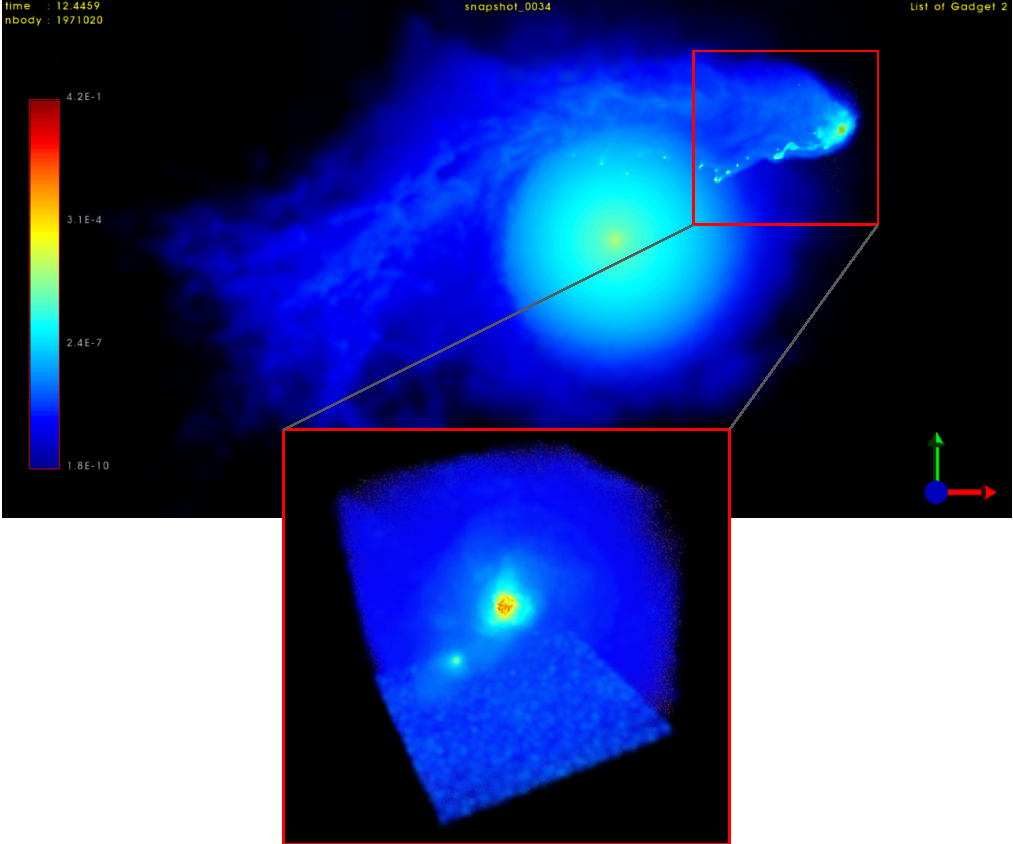
\includegraphics[width=\textwidth]{MovingBox.pdf}
 \caption{An illustration, top panel, of a full fledged simulation of a dwarf galaxy with a Fornax-like cluster. 
 Colors show the gas density \citep[using the \texttt{glnemo2} software][]{Lambert2012}.
 Note the number of particles involved, almost 2 millions.
 The moving box technique, represented in the boxy inset, allows to concentrate resources on the interesting part of the simulation.
 Also, at the dwarf-cluster interface an increased resolution is possible, better resolving the stripping.}
 \label{fig:MovingBox}
\end{figure}

We have opted to use the moving-box technique described by \citet{Nichols2015} and further developed by \citet{Hausammann2019}.
As shown in Figure~\ref{fig:MovingBox}, we enclose the MoRIA dwarf in a $60$~kpc wide moving simulation box, as in a wind tunnel simulation.
Gas is injected from the open ``front" side of the box, which always points in the dwarf's direction of motion. Its density and temperature vary with position, as discussed below in Section \ref{sec:fornax_sim}.
This mimics the hot wind of the cluster halo gas as it streams past the orbiting dwarf galaxy.
Also, additional fictitious forces on the particles are included to take into account the rotation and orbital motion of the moving box.
This allows us to simulate the combined effects of tidal forces and ram-pressure stripping \citep[as studied by][]{Mayer2006} which are acting simultaneously on the dwarf without the necessity of simulating a galaxy cluster worth of intra-cluster gas.
% A typical simulation snapshot contains around $150$k gas particles and $16$k star particles, each with a mass of $4000$~\Msun{}.

\subsection{Quaternions}
For completeness, we briefly introduce quaternion algebra.
Following \citet{Graf2008}, a quaternion is a set of four parameters, a real value $q_0$ and three imaginary values $q_1\vect{i},q_2\vect{j},q_3\vect{k}$ with $q_1,q_2,q_3 \in \mathbb{R}$ usually represented as:
\begin{equation}
 \quat{q} = q_0 + q_1\vect{i} + q_2\vect{j} + q_3\vect{k}.
\end{equation}

The core of quaternion algebra is Hamilton's rule for multiplication of the imaginary units $\vect i, \vect j, \vect k$:
\begin{equation}
 \vect i^2 = \vect j^2 = \vect k^2 = \vect{ijk} = −1,
 \label{eq:hamilton_quaternion}
\end{equation}
from which a complete set of non commutative multiplication rules can be derived.
In fact, noting for example that by left multiplying the last equality in eq. \eqref{eq:hamilton_quaternion} by $\vect i$: $\vect i\,\vect{ijk}=-\vect{jk} = -\vect i$, the product of the imaginary parts are:
\begin{equation}
 \vect{ij} = \vect k, \, \vect{jk} = \vect i, \, \vect{ki} = \vect j.
 \label{eq:hamilton_quaternion_mixed}
\end{equation}

Another useful representation of a quaternion is as a pair $\quat{q} = (q_0, \vec q)$ of a scalar part $q_0\in \mathbb{R}$ and a vector part $\vec q \in \mathbb{R}^3$ (also called real and imaginary parts, respectively).
\footnote{Only in this section, to distinguish between quaternions and three dimensional-space vectors, we'll use boldface $\quat{q}$ for quaternions and $\vec q$ for $\mathbb{R}^3$ vectors. In the other sections the difference among the two will be clear from the context.}
Its conjugate~$\conj{\quat{q}}$ is defined as:
\begin{equation}
 \conj{\quat{q}} = (q_0, -\vec q),
 \label{eq:conjugate}
\end{equation}
and its norm as:
\begin{equation}
 \norm{\quat{q}} = \sqrt{q_0^2+q_1^2+q_2^2+q_3^2}.
\end{equation}

From eqs. \eqref{eq:hamilton_quaternion} and \eqref{eq:hamilton_quaternion_mixed} in particular we can write the general formula for the non commutative quaternion multiplication, i.e. given two quaternions $\quat{q}$ and $\quat{p}$:
\begin{equation}
 \quat{q} \,\quat{p} = (q_0 p_0 - \vec q \vdot \vec p, \, q_0 \vec p + p_0 \vec q + \vec q \cross \vec p).
 \label{eq:quaternion_multiplication}
\end{equation}
From \eqref{eq:conjugate} it follows that $\quat{q} \,\conj{\quat{q}} = \norm{\quat{q}}^2 \equiv (\norm{\quat{q}}^2, \vec 0)$. For unit quaternions ($\norm{\quat{q}} = 1$), we can write $\conj{\quat{q}} = \quat{q}^{-1}$.% because $\vect 1 \equiv (0$.

\paragraph{Quaternions and rotations} Unit quaternions are also called \emph{rotation quaternions}.
They can be used to completely describe a rotation of an angle $\varphi$ around the axis $\vec q$.

Let's consider a unit quaternion $\quat{q}$. It can be always written as:
\begin{equation}
 \quat{q} = (q_0, \vec q) = (\cos \frac \varphi 2, \sin \frac \varphi 2\, \hat n), \quad \text{with } \norm{\hat n}=1,
\end{equation}
where $\hat n \equiv \vec q/\norm{\vec q}$ is the versor of $\vec q$.\\
A vector in three-dimensional space $\vec x \in \mathbb R^3$ can be expressed as a \emph{pure quaternion}, a quaternion with no real part: $\vect x = (0, \vec x)$.
% It can therefore multiplied by a quaternion using relation \eqref{eq:quaternion_multiplication}.

The vector $\vec x'$ resulting from the rotation of $\vec x$ of an angle $\varphi$ around the axis $\vec q$ is given by the conjugation operation:
\begin{equation}
\vect x' = \conj{\quat{q}}\, \vect x \, \quat{q} 
\end{equation}
where $\vect x' = (0, \vec x')$ \citep[for a proof, see e.g.][sec. 1.4]{Graf2008}.

In the following sections we'll write equations that involve the rotation a quaternion by a vector.
With a slight abuse of notation we will write directly $\vect x' = \conj{\quat{q}}\, \vect x \, \quat{q}$, considering that the vector indicated in boldface $\vect x$ should be understood to be the pure quaternion $(0, \vec x)$.% given that it will be clear from the context what is a quaternion (mainly just $\quat{q}$).



\subsection{Velocity and acceleration of the particles in the moving box}
\paragraph{Reference frames}
\begin{figure}[H]
 \centering
 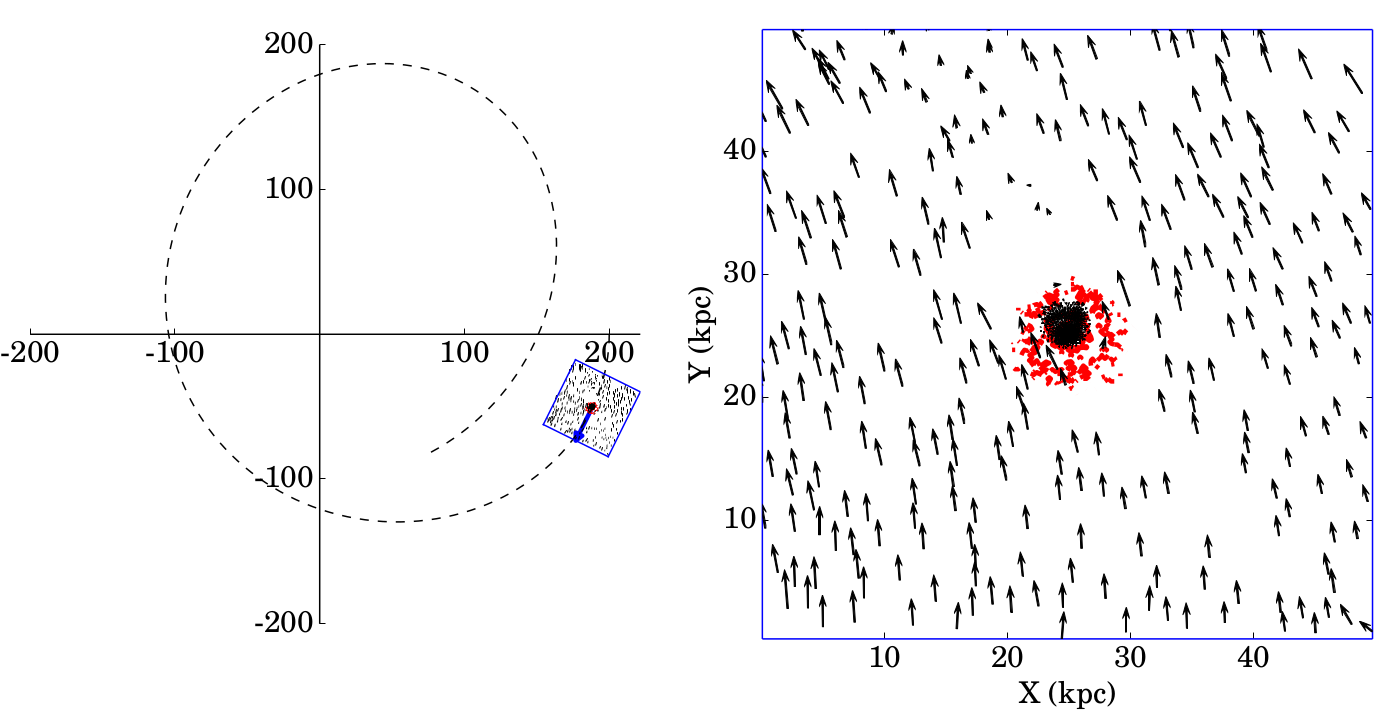
\includegraphics[width=\textwidth]{moving_box_nichols.png}
 \caption{From \citet{Nichols2015}. On the left it is shown the the moving box trajectory. The blue arrow represents the instantaneous box (and therefore dwarf galaxy) velocity.
 On the right, gaseous particles are injected from the bottom side of the box. In red, dark matter density contours, and arrows indicate the wind particles velocity.}
 \label{fig:mb_nichols}
\end{figure}
In a moving box simulation we define the inertial reference frame where the cluster is at the origin.
Relative to that, the box moves and rotates, as shown in Figure \ref{fig:mb_nichols}.
Following the convention in \citet{Nichols2015}, capital letters are used for vectors in the inertial frame whereas small letters for vectors in the moving box (rotating frame).

Let $\quat{q}$ be the quaternion which at each point in time maps the~$-y$ axis of the rotating reference frame to the direction of the velocity of the box in the inertial frame, $\Vp$.
Therefore, a vector $\vect X$ in the inertial frame, corresponds to $\vect x = \conj{\quat{q}}\, \vect X \,\quat{q} $ in the rotating frame.
% To represent the correct rotations, at each moment the quaternion  the moving box is computed.
A fixed point inside the moving box is taken as a reference point, the so called \emph{pivot}, whose coordinates relative to the box are $\xp$ and its velocity and acceleration in the inertial frame relative to the cluster are denoted with $\Vp$ and $\Ap$, respectively.
The \emph{pivot} represents the position in the box of minimum specific energy (the average position of the 64 particles with minimum total potential and kinetic energy) at the start of the simulation and is used to track the velocity and the acceleration of the box.

For a generic particle, the velocity in the moving box reference frame is:
\begin{equation}
 \label{eq:mb_velocity}
 \vect{v} = \quat{q} \,\Vp\, \conj{\quat{q}} - \vect \omega\cross(\vect x -\xp),
\end{equation}
and its acceleration:
\begin{equation}
 \label{eq:mb_acceleration}
 \vect{a} = \quat{q} \,\Ap\, \conj{\quat{q}} - 2\,\vect \omega \cross \vect{v} - \vect\omega \cross ( \vect \omega \cross (\vect x-\xp)) - \dot{\vect \omega}\cross(\vect x -\xp).
\end{equation}


\subsection{Critically damped oscillator}
The acceleration of the pivot point is due mainly to the gravitational attraction of the cluster.
The dwarf galaxy experiences also a low intensity drag due to the gas impinging the galaxy.
In our simulations, this drag is always $<5\%$ than the gravitational acceleration.
In order to keep the galaxy at the center of the box, an \emph{ad~hoc} corrective acceleration $\Ap^{hoc}$ is added to it as it moves.
This translates to adding an acceleration term to the pivot $\Ap = −\grad \Phi(\vect X_\mathrm p) + \Ap^{hoc}$.

In \citet{Nichols2015}, the correction term is intended to become zero when not needed.
In practice, the $64$ particles with lower total energy (kinetic plus potential) are tracked at each timestep and their average position ($\vect X_{64}$) is taken as the center of the galaxy.
The goal of the ad hoc acceleration is to move the box to follow the center of the galaxy and so compensate the drift of these particles from the pivot.
In the original implementation, $\Ap^{hoc}$ is put to zero as soon as the velocity of the central low energy particles is again directed towards the pivot point (i.e. $(\vect X_{64}-\vect X_\mathrm p) \vdot (\vect{V}_{64} - \Vp) < 0$).
This understandably is done to minimize the total impulse due to the ad hoc term.
But this sudden acceleration removal can cause active particles during the numerical time integration to be kicked away unnaturally, because of the particle acceleration in equation \eqref{eq:mb_acceleration}.
An improvement in our implementation of the moving-box method is the use of a critically damped oscillator for the \emph{ad~hoc} acceleration.
\begin{equation}
 \Ap^{hoc} = 2\,\zeta\omega_0 \Vp + \omega_0^2 \vect X_\mathrm p,
\end{equation}
where $\omega_0$ is the undamped angular frequency of the oscillator, and $\zeta$ the damping ratio.

We start by noting empirically that for our typical galaxy size a sufficient acceleration requires that $\omega_n^2\approx 10$ Gyr$^{-2}$.
Given that we want to dump the oscillation as fast as possible. We use a critically damped oscillator  for which $\zeta = 1$. Therefore the viscous coefficient $2\,\zeta\omega_0$ is simply $6.3$~Gyr$^{-1}$.
A typical behaviour of the \emph{ad~hoc} acceleration is shown in Figure \ref{fig:adhoc}.

\begin{figure} % TODO include adhoc figure
\centering
%  \includegraphics[width=0.8\textwidth]{adhoc.png}
\caption{Adhoc acceleration relative to the total gravitational acceleration of the simulation ID 68 with pericenter 150 kpc.}
\label{fig:adhoc}
\end{figure}


\subsection{Recovering the correct kinematics from a moving box simulation}
\label{sec:correct_kinematics}
We are interested in finding the expression of the velocity $\vect{V}$ in the inertial frame at a certain position $\vect{x}$ in the moving box, knowing its velocity in the rotating frame $\vect{v}$. 
Let $\vect{\Omega}$ be the angular velocity of the box in the inertial frame which can be computed as:
\begin{equation}
 \vect{\Omega} = {(\Vp\cross\Ap)}/{\Vp^2}.
\end{equation}
In the rotating frame the angular velocity of the box can be expressed as:
\begin{equation}
\vect \omega = \conj{\quat{q}}\, \vect{\Omega}\, \quat{q}.
\end{equation}
We can then transform back from rotating to inertial coordinates by applying this transformation:
\begin{equation}
\vect{V} = \Vp + \quat{q} \, \left(\vect{v} + \vect{\omega} \cross (\vect{x}-\xp)\right) \,\conj{\quat{q}}
\end{equation}
where $\mathbf x$ and $\mathbf v$ are position and velocity of the particle in the rotating frame, respectively, and $\mathbf V$ its velocity in the inertial frame. % For simplicity in the following we don't take into account $\Vp$ since its contribution to the line of sight velocity is negligible.

\subsection{Injecting and removing particles in the moving box}
The wind of the moving box is due to particles belonging to the cluster injected with correct velocity, density and temperature in the box.
We assume the cluster gas to have the density and pressure of the Fornax cluster as described by \citet{Paolillo2002} and in \refsec{sec:ICM}. We also assumed zero metallicity and $\alpha-$abundance.

The cluster gas is injected using a sort of ``cartridge'' of particles previously computed as a unit sized cubic glass structure of $N_{\text{glass}} \approx 18000$ particles.
The glass is generated from a random distribution of particles letting them evolve in a periodic box with negative gravitational attraction (effectively being a repulsive force).
The resulting low energy distribution of particles guarantees a low probability of injecting dense clumps of particles which would have high kinetic energy once released.

At each timestep the correct amount of new particles to be injected is taken from the ``cartridge''.
The number of particles belonging to the cluster $N_c$ would be the correct amount to fill up the entire box of size $L$ with the correct cluster density $\rho_c(r)$ at the instantaneous orbital radius $r$.
Therefore they respect the relation:
\begin{equation}
 N_c m_g = \rho_c(r) L^3.
\end{equation}

The fraction of particles to be taken from the cartridge is then: $\xi=\dfrac{N_c}{N_{\text{glass}}}$. The number of particles in the glass should be chosen in order for $\xi\leq1$.
A slice of the glass unit cube is then taken in such a way that its depth is 
\begin{equation}
\frac{\norm{\Vp}\Delta t}{L} \sqrt[3]{\xi},
\end{equation}
and width and length are both $\sqrt[3]{\xi}$. The density and the temperature of the new particles are set according to the quantities instantaneous radial distance of the galaxy, the pressure and energy computed using the equation of state.
By construction the new particles have velocity $\norm{\Vp}$ directed towards the local moving box axes $+y$.

If a particle of any kind gets closer than $L/100$ from the rear edge of the box, it gets deleted.
The lateral edges of the box are periodic for gas particles, to keep a constant flow around the galaxy, but dark matter or stellar particles are removed if closer than $L/500$ from any lateral edge of the box.
This process has been fine tuned and extensively tested by \citet{Nichols2015} and \citet{Hausammann2019}.

% It's worthwhile noting that the implementation the deletion or creation of particles in distributed code as the \textsc{Gadget-2} is not a trivial task.
% The arrays representing the particles undergo this kind of algorithm.
% In the end, a rolling 

\section{Simulating the Fornax cluster environment}
\label{sec:fornax_sim}

\subsection{Cluster model}

\subsubsection{Dark matter}
The simulations take into account both ram pressure stripping and the tidal interaction with the cluster.
The latter is simulated as a single spherically symmetric static NFW potential profile \citep{Navarro1996} with mass $M~=~10^{14}$~\Msun{} \citep{Drinkwater2001a}:
\begin{equation}
    \Phi(r) = \frac{G M}{r} \frac{\log(1+r/R_s)}{\log(1 + c) - \frac{c}{1+c}}
\end{equation}
with scale length $R_s = 120$ kpc and $c=8.15$ derived from scaling relations in e.g. \citet{Gentile2004, Wechsler2002}:
\begin{equation}
    c \simeq 20 \left(\frac{M}{10^{11} \text{\Msun{}} }\right)^{-0.13}, \qquad
    R_s = \frac 1 c \left(\frac{M}{\frac 4 3 \pi 200 \rho_c}\right)^\frac 1 3,
\end{equation}
with $\rho_c = 127.3$~\Msun{}~kpc$^{-3}$ the critical density of the universe at $z=0$ for a cosmology with Hubble constant $h=0.67$ and $\Omega_m = 0.31$ \citep{Planck2015}.
The cluster virial radius of the model is $R_{\mathrm{vir}} = c R_s = 978$~kpc.

\subsubsection{ICM} \label{sec:ICM}
Following \citet{Paolillo2002}, we use the superposition of three spherically symmetric beta-models, $\rho(r) = \rho_0 (1 + (r/r_0)^2 )^{-3\beta/2}$, to construct the gas density profile in the Fornax cluster, as shown in Figure \ref{fig:profiles}.
They identify three contributions to the hot gas distributions: a central component (dominating for $r<5''$), coincident with the optical galaxy NGC1399; a less dense and more extended galactic component ($50''<r<400''$); and a cluster component ($r>400''$).
We assume the gas to be in hydrostatic equilibrium with temperature $T(r)$ computed as:
\begin{equation}
   T(r) = \frac {m_p}{k_B \rho(r)} \int_r^\infty \rho(r') \frac{GM(r')}{r'^2} \mathrm{d} r'
\end{equation}
where $M(r)$ is the mass of the gas, stars and dark matter beyond radius $r$, $m_p$ is the proton mass, $G$ and $k_B$ the gravitational and Boltzmann constants.

\begin{figure}
\centering
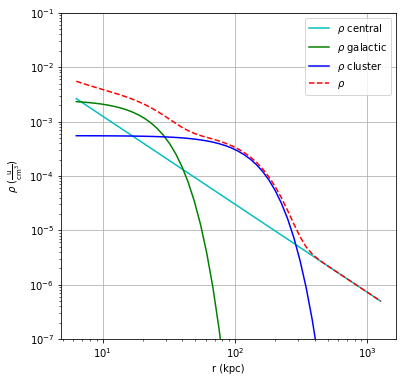
\includegraphics[width=0.8\textwidth]{PaolilloRho.png}
\caption{Gas density profile $\rho(r)$ of the  Fornax Cluster model as a superposition of three beta models from measurements described in \citet{Paolillo2002}, from which we also adopt the nomenclature for the different beta models.
}
\label{fig:profiles}
\end{figure}

These two radial profiles allow us to inject particles with the proper density and temperature in the moving box, hence recreating the environmental condition of the cluster as the dwarf orbits through it.

\subsection{Simulation parameters}
We carried out a set of simulations starting from five MoRIA models of late-type galaxies taken at $z = 0.5$.
The overall goal in setting up the simulations is to study the evolution of late-type galaxies in a cluster environment.
The choice of the redshift of infall has been motivated by the fact that the number of red dwarfs in the Fornax cluster has increased significantly since $z = 0.5$ \citep{Stott2007, DeRijcke2010}.
That indicates that the conversion of late-type to early-type dwarfs (and hence the acquisition of late-type dwarfs by clusters) is probably a recent event.

We selected dwarfs models covering the stellar mass range of $10^{7.5}-10^{9}$ and we injected each of them on 5 different orbits with pericenter distances of $50, 100, 150, 200,$ and $300$~kpc and with a fixed apocenter of 800 kpc.
The starting point of the infall is always at a radial distance of 600~kpc.
We chose a lower radial distance of the starting position with respect to the virial radius given the very low cluster density in that region and the low orbital velocity of the dwarf near apocentre.
In this way, simulations could be concentrated on the infall and the pericenter passages of the simulated dwarfs.
We evolved the galaxies for $5.5$~Gyrs up to $z=0$.
The initial stellar masses are reported in Table \ref{tbl:sim}.
All simulations presented in this paper, at time of injection have exponentially declining SB profiles with Sersic index around 1.0.
Every $10$~Myr a snapshot is saved, yielding around 560 snapshots for each simulation.
This high snapshot cadence has proven to be important for the following analysis (see \refsec{sec:morphological_quest}).
Adhering to the simulation goal of following the evolution of a gas-rich late-type dwarf in a Fornax-like cluster, the initial snapshot of the most massive dwarf (ID 41) has been taken at $z=0.4$ because at $z=0.5$ it was still undergoing a major merger event.
This is equivalent to having this galaxy falling into the cluster more recently.
No sizeable effect has been noted in simulations results highlighting a different behaviour with respect to the other galaxies \citep[which underwent their last merger before infalling to the cluster at $z=0.5$, see e.g.][]{Cloet-Osselaer2014}.
This has had the only implication of a lower number of snapshots used in the technique explained in \refsec{sec:morphological_quest}, but, as we shall see in the following, given that first pericenter passage turns out to be the most significant orbital phase, no notable bias is expected.

\begin{table}
\centering
\footnotesize
\begin{tabular}{cx{1.3cm}x{0.5cm}x{0.8cm}x{0.7cm}x{0.4cm}x{1.4cm}}
\toprule
Sim ID & $\log_{10}$(M$_\star$)\newline(M$_\odot$) & $R_e$ \newline (kpc) & $\sigma_\star$ \newline (km/s)\\
\midrule
  62 &  6.66 &  0.8 &  11.4 \\%&  -11.8 &  0.5 &  25.8 \\
  71 &  7.58 &  1.9 &  21.9 \\
  68 &  7.96 &  2.6 &  15.6 \\
  69 &  8.04 &  2.3 &  24.6 \\
  41 &  8.78 &  1.7 &  30.4 \\
\bottomrule
\end{tabular}
\caption{Features at time of infall ($z=0.5$) of the selected MoRIA dwarf models used in this work}
\label{tbl:sim}
\end{table}


\section{Only tides simulations}
In order to isolate the effects of the tides and of the ram pressure, we performed some representative simulations without the cluster gas.
% These hypothethical simulations show...

In Figure~\ref{fig:gas_no_gas}, are shown the typical tidal tails due to tides...

\begin{figure}[ht]
 \centering
%  \includegraphics[width=0.8\textwidth]{gas_no_gas.png}
 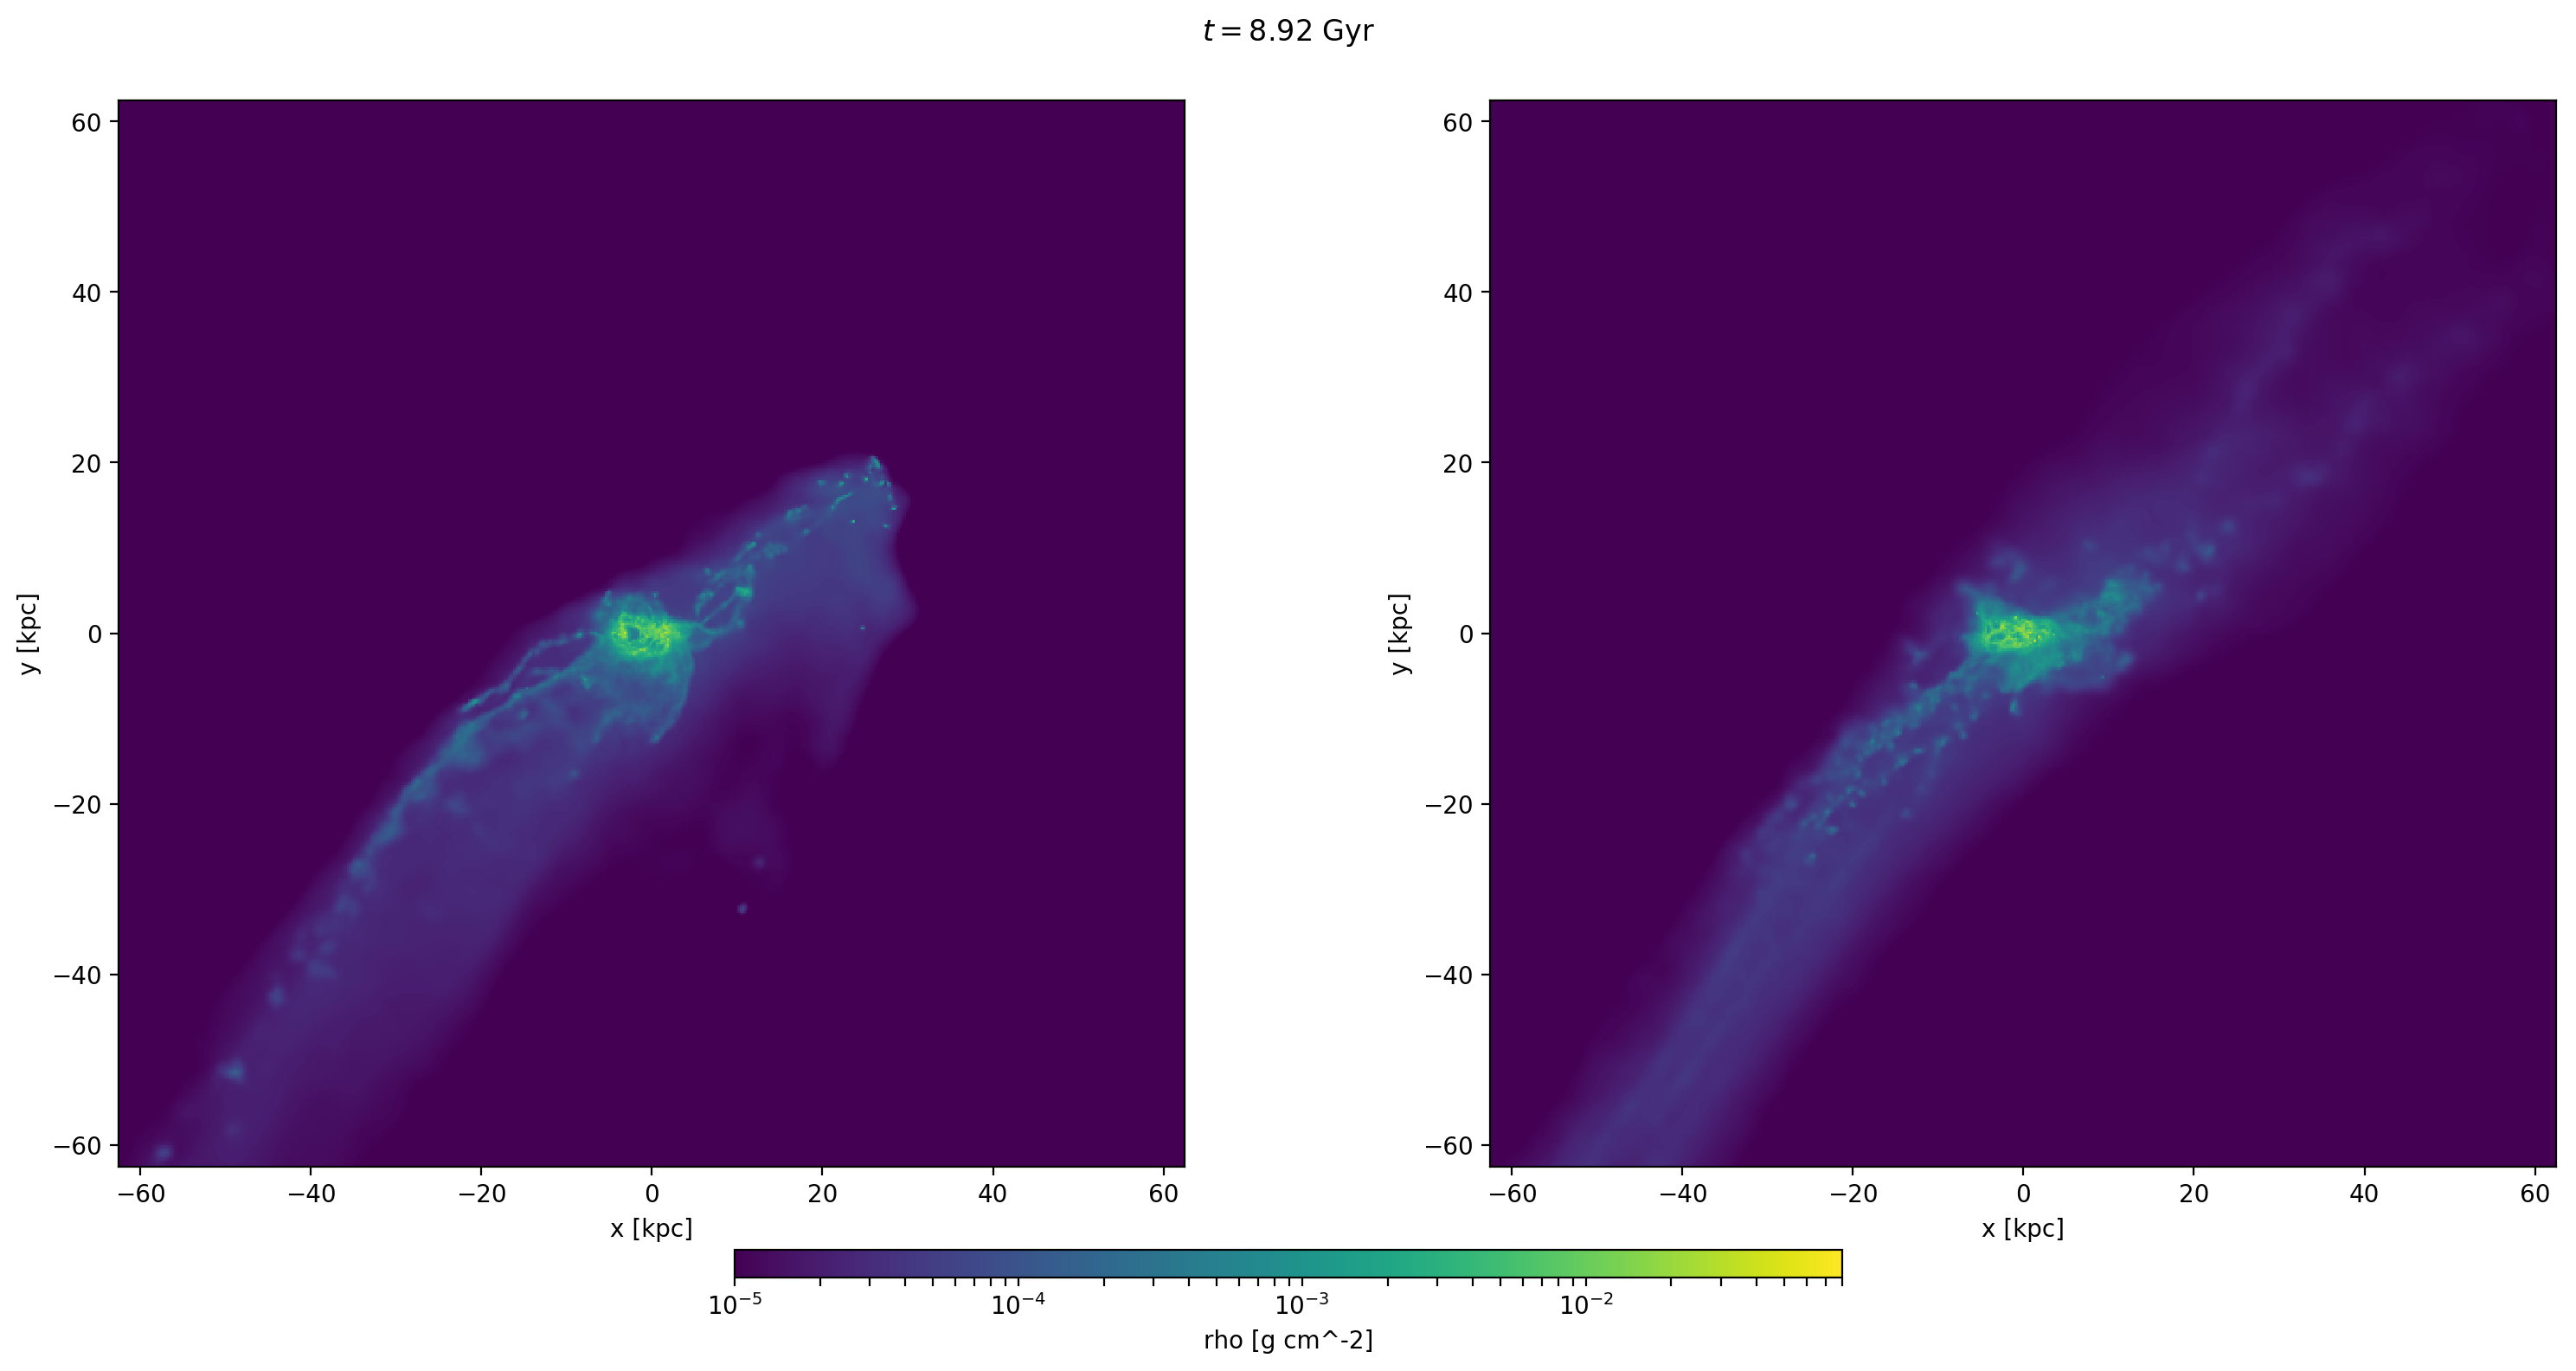
\includegraphics[width=\textwidth]{stripping2.png}
 \caption{Projected gas density map of a galaxy orbiting a Fornax-like cluster.
 On the right, the gas interacting with the dwarf creates a wake and a single tidal tail is formed; on the left a snapshot without cluster gas: two tidal tail are shown.}
 \label{fig:gas_no_gas}
\end{figure}
